\subsection{Deep Learning}
Deep Learning is a class of machine learning systems whose goal is to extract relevant features from a distribution of data. On an abstract level, Deep Learning systems take inspiration the structure of human biology, with multi-layer structures of nodes (Neurons): each layer might be thought of as a section of a brain recognizing a very specific element, and when all layers work in unison they can recognize and act upon high level features and categories.

%Deep learning is used in many fields, and has achieved notable results in fields such as Computer Vision, Image Recognition and Natural Language Processing.%REFERENCE

Deep Learning Systems are particularly useful because of their ability to extract high level features from data, especially features that are hard to define algorithmically by humans.

Another peculiar features of such network is that no-one really knows exactly how the machine learns. There has been such research trying to understand what exactly each layer does and what exactly it learns, but this is still an open question.\newline %REFERENCE.
Because of the number of variables involved, it is hard to predict results might derive from a change in the initial condition; as a consequence of this uncertainty, the process of working with Deep Learning system is one of incremental change and experimentation. 

Figure \ref{fig:DNN} shows the typical structure of a Deep Neural Network:
\begin{figure}[H]
\centering    
\begin{neuralnetwork}[height=8]
\newcommand{\x}[2]{$x_#2$}
\newcommand{\y}[2]{$y_#2$}
\newcommand{\hfirst}[2]{\small $h1_#2$}
\newcommand{\hsecond}[2]{\small $h2_#2$}
\inputlayer[count=4, bias=false, title=Input Layer, text=\x]
\hiddenlayer[count=8, bias=false, title=Hidden Layer 1, text=\hfirst] \linklayers
\hiddenlayer[count=8, bias=false, title=Hidden Layer 2, text=\hsecond] \linklayers
\outputlayer[count=4, title=Output Layer, text=\y] \linklayers
\end{neuralnetwork}
\caption{An example of a Deep Neural Network}\label{fig:DNN}
\end{figure}
As we can see in the example above, a neural network is composed of an Input Layer, a number of Hidden layers and an Output layer.
Speaking in general terms, the input layer receives the chunk of data to be processed, the hidden layers operate on the input sequentially, and the output layer is where the system expresses what it believes the data to mean.

Training of a neural network is composed of two distinct phases: the \emph{Feed Forward} phase and the \emph{Back-Propagation} Pahse: In the feed forward phase the network processes the current data and comes to a result, then the networks computes the Error (or how much the result it had come to deviated from the expected results). The network then takes the error value and propagates it backwards by adjusting 
the weights of the connections between each neuron in the different layers, in an effort to reduce the error
Once both phases are completed the network has completed an iteration. The next batch of data is then introduced and the process begins anew.

In this coming section we will cover two types of Deep Learning Neural Networks that are relevant in this paper: \emph{Recurrent Neural Networks} (RNNs) and  \emph{Generative Adversarial Networks} (GANs).
%\clearpage

\subsubsection{Recurrent Neural Networks}
Recurrent Neural Networks are the simpler of the two network architectures; they are a kind of neural network specialized in working with data that has a temporal component.
For instance if the network needs to predict the next letter or word in a sentence, it needs to know what came before. Another example might be a neural network that scales or edits videos, where the action to take on any given frame might be dependent on the frames that came before.

The precise method the network uses to keep track of temporal elements is rather complex, but can be briefly summarized by saying that each neuron in the network holds a state, and that each iteration a neuron's state from the previous iteration is fed as input to itself in the current iteration along side the current data to be processed.
This creates a feedback loop, whereby at any given point the calculation performed by each neuron are influenced by previous events.

\begin{figure}[H]    
\centering
\begin{tikzpicture}[shorten >= 1pt, node distance = 2cm, on grid, auto, square/.style={regular polygon, regular polygon sides = 4}]
\node[](0){};
\node[below of = 0](1){};
\node[below of = 1] (2){};

\node[state, right of = 1](N1){$H1_{(t)}$};
\node[state, right of = N1](N2){$H2_{(t)}$};
\node[state, right of = N2](output){$O$};

\draw[-]   (0) edge node{$x_i$} (N1)
            (2) edge node{$x_i$}(N1)
            (N1) edge (N2)
            (N2) edge (output);
\end{tikzpicture}
\begin{center}
Iteration number 1 $t=1$
\end{center}
\end{figure}

\begin{figure}[H]
\centering    
\begin{tikzpicture}[shorten >= 1pt, node distance = 2cm, on grid, auto, square/.style={regular polygon, regular polygon sides = 4}]
	\node[](0){};
	\node[below of = 0](1){};
	\node[below of = 1] (2){};
	
	\node[state, right of = 1](N1){$H1_{(t)}$};
	\node[state, right of = N1](N2){$H2_{(t)}$};
	\node[state, right of = N2](output){$O$};
	
	\draw[-]   (0) edge node{$x_i$}(N1)
	(2) edge node{$x_i$} (N1)
	(N1) edge[loop above] node{$H1_{(t-1)}$} (N1)
	(N2) edge[loop above] node{$H2_{(t-1)}$} (N2)
	(N1) edge (N2)
	(N2) edge (output);	
\end{tikzpicture}
\begin{center}
Iteration number 2 $t=2$
\end{center}
    \caption{A simplified representation of a node in a Recurrent Neural Network}\label{fig:rnn_neuron}
    
\end{figure}
%\clearpage
Figure \ref{fig:rnn_neuron} illustrates the working of a RNN neuron: taking picture \ref{fig:DNN} as a starting point we can see the feedback loop of an RNN node at work.
The first picture shows the state of three nodes in the network on iteration 1: During the feed forward phase the first neuron in the hidden layer one receives input $x$ from the input layer, processes it and passes it on to the consecutive layers; after processing, each hidden neuron saves its working values, and those values form the node's state.  

In the next iteration (shown in the second picture) the process repeats, but this time the  H1 node receives not only input from $x$, but also its previous state as input; it processes the combined values and passes it on to H2, which undergoes the same procedure.

Through this mechanism, the network can better retain knowledge of features from past samples of data, and yield better results.
However this also highlights a potential problem: because each node is only fed its previous state with each successive iteration, as the training process continues the network will develop a bias towards more recent samples of data.
 The cyclical nature of the feed-forward means that at any given iteration the network will retain memory of the initial stages of training, but the influence of those early iterations will wane with time as the network adapts and changes when presented with new data. This phenomenon is usually called 'Gradient Decay'\\
% LSTM might be waaay too much detail. Also fuck its a *masive over-simplificatin*
For some particular tasks such as Natural language generation, gradient decay can significantly influence the final results.

% setup is not enough, since as time goes on the network will develop a bias towards features present in more recent iteration; the influence of data from the older iteration will degrade over time, and the system will slowly tend to 'forget' features and patterns it learned at the beginnning: when it is then presented with new data it has never seen before, thi bias can pose a problem.

%To dampen the effects of this bias one might employ Long-Short Term Memory cells (LSTM), a special kind on RNN neuron which can dynamically rank new information (and by extention, the content of its state) based on its relevance. LSTM ensures that important data is retained regardless on when it was learned, and thus diminishes the effect of the base RNN bias.\newline
%It should be noted however that LSTM does not constitute a straight upgrade from the plain RNN architecture: it may be beneficial in certain cases, but decremental in others.

\subsubsection{Generative Adversarial Networks}
Generative Adversarial Networks are a more complex architecture, composed of two discrete neural networks that are in competition with each other.

The system works by employing a generative network $(G)$ and a discriminator network $(D)$:

\begin{figure}[H]
\centering
    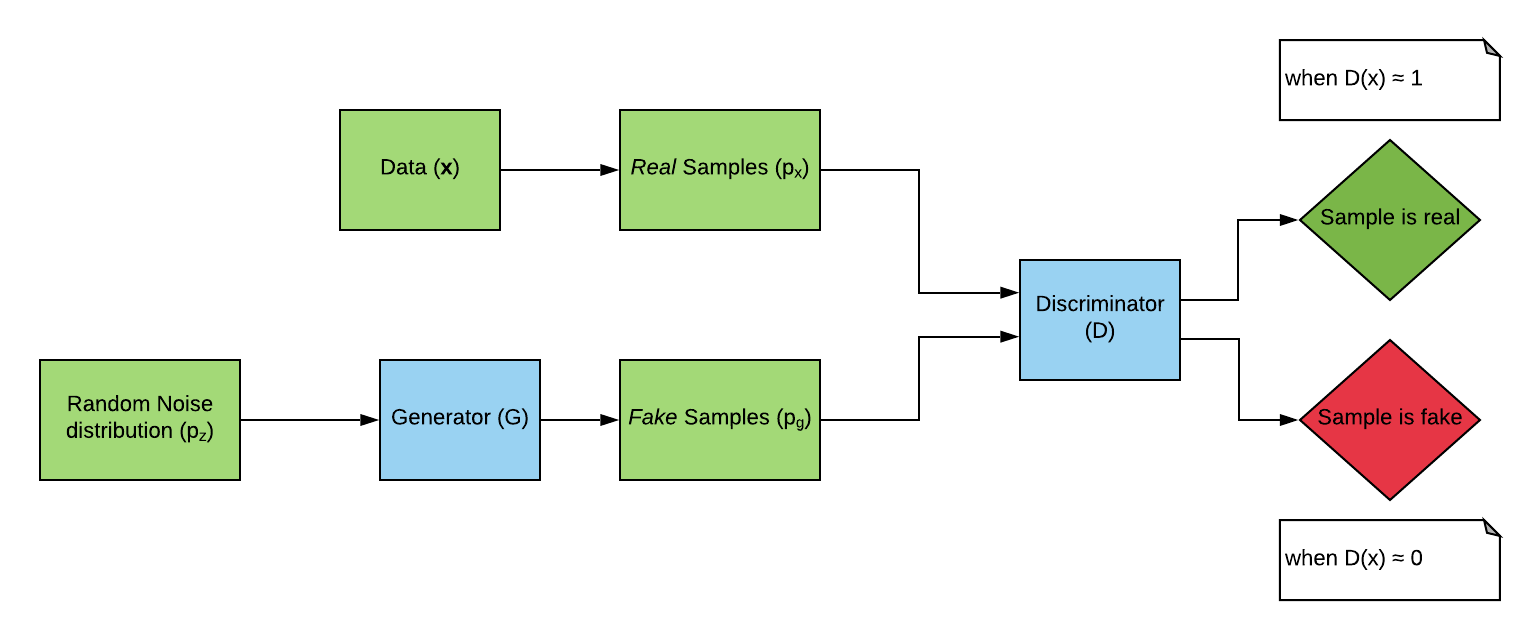
\includegraphics[scale=0.60]{figures/GAN_v2.png}
    \caption{An illustration of the general structure on a Generative Adversarial Network}
    \label{fig:gani-diagram}
\end{figure}    

$G$ generates samples from a random noise distribution $p_z$. We call the resulting data distribution $p_g$; $D$ is fed both data from the training set ($x$) and the output from $G$ ($p_g$), and it's task is to figure out whether any given sample comes from the data (it belongs to $p_x$) or has been generated from $G$ (it belongs to $p_g$). In layman terms, we might say that it is $D$'s job to tell 'real' samples from 'fake' ones.

%The feedback from $D$ is factors into the Error function and helps $G$ improve, and the goal is to train untill $D$ is no longer able to tell the two inputs apart.

%As Goodfellow et al. \cite{Goodfellow2014} explain in their paper, $D$ is trained to maximize the likelihood of assigning the correct label to both data samples and samples from $G$; The generative network in turn is encouraged to generate data that is as similar as possible to the underlying distribution: this creates a race of sorts between the two networks, and a beneficial feedback loop between the two.

Goodfellow et al.\cite{Goodfellow2014} explain the interplay between the two networks as a min-max game: the goal of $D$ is to maximize the likelihood of guessing correctly, while the goal of $G$ is to minimize that same likelihood (or to put it another way, $G$ wants $D$ to make more mistakes): the reason for this is that by minimizing the likelihood of $D$ guessing correctly, we are implicitly telling $G$ to generate samples as close as possible to the input data.

Simply put, the two networks are trying to out-smart each other: every time $D$ tries to spot the 'fake' samples from $p_g$, while $G$ tries to improve more and more to make $D$'s job harder.

The output of $D$ is a single value between 0 and 1 expressing the network's confidence on whether a sample came from $x$; Values of $D(x)$ closer to 1 tend towards assigning a sample to the input data distribution.
Ideally, this race/competition between the two networks comes to an end when the output $D(x)$ stabilizes on $D(x)=0.5$, meaning that $D$ is no longer able to tell the two distributions apart.

%If we trained the network correctly, this will also mean that $p_x=p_g$, and thus we can conclude the training.
This also tells us that if we had infinite resources (both in  data samples and computing resources), we could train until $D(x)=0.5$ and $p_x=p_g$, giving us an output of $G$ that is indistinguishable from the input data.

One important thing to note is that we do not show $G$ any of the input data at any point: all that $G$ has access to is a random noise distribution and the error value for $D$; the Generator has to slowly shape that noise into data resembling the Discriminator's input, by using Gradient Descent.  

The process described above can be formalized in the following general equation:
\begin{equation}
 \min\limits_{G} \max\limits_{D} V(D,G)=\mathbb{E}_{x\sim p_{data}(x)}[\log{D(x)}]+\mathbb{E}_{z\sim p_z(z)}[\log{(1-D(G(z)))}] 
\end{equation} 

Because operation of the network relies on this tight feedback loop between $D$ and $G$, one needs to pay close attention to how quickly each network learn.
The idea, as the authors in \cite{Goodfellow2014} point out, is to have a certain number of iterations of $D$ before we go ahead and adjust the Error for $G$; Conceptually, we might think of this as giving $D$ enough time to tell the real from the fake data reliably (or try), before iterating $G$ to counter $D$'s current strategy.

The original paper indicates this ratio with $k$, and notes that increasing it grows the required computation significantly. In their experiments the authors used a $k$ value of one for performance reasons, while PassGAN defaults to a $k$ value of 10\cite{PassGAN}.

\paragraph{PassGAN}


